\subsection*{一、兩角強度比隨光學厚度的變化}
本研究以
\[
    C = \frac{I(30^\circ)}{I(125^\circ)}
\]
作為角度分布指標。表一整理兩種粒徑在六個光學厚度下的實驗值與蒙地卡羅模擬值。當 $\tau$ 由 $0.5$ 增加至 $8$，$0.492\,\mu\mathrm{m}$ 微球的實驗 $C$ 由 $12.06$ 降至 $1.92$，$2.16\,\mu\mathrm{m}$ 微球則由 $21.71$ 降至 $3.81$。各光學厚度下，較大粒徑的 $C$ 均較高，約為較小粒徑的 $1.6$ 至 $2.4$ 倍。圖~\ref{fig:C-tau} 上圖為兩者隨 $\tau$ 的變化，下圖為實驗／模擬比值。

\begin{table}[H]
    \centering
    \caption{實驗與蒙地卡羅模擬的兩角強度比 $C$}
    \label{tab:result-c}
    \small
    \renewcommand{\arraystretch}{1.2}
    \begin{tabular}{ccrrr}
        \toprule
        粒徑 ($\mu$m) & $\tau$ & 實驗 $C$ & 模擬 $C$ & 實驗／模擬 \\
        \midrule
        0.492 & 0.5 & $12.06 \pm 0.52$ & 14.02 & $0.86 \pm 0.04$ \\
        0.492 & 1   & $10.85 \pm 0.49$ & 10.34 & $1.05 \pm 0.05$ \\
        0.492 & 2   & $7.47 \pm 0.31$  & 6.32  & $1.18 \pm 0.05$ \\
        0.492 & 4   & $3.93 \pm 0.06$  & 3.14  & $1.25 \pm 0.02$ \\
        0.492 & 6   & $2.62 \pm 0.04$  & 2.00  & $1.31 \pm 0.02$ \\
        0.492 & 8   & $1.92 \pm 0.02$  & 1.49  & $1.29 \pm 0.01$ \\
        \midrule
        2.16  & 0.5 & $21.71 \pm 1.61$ & 25.78 & $0.84 \pm 0.06$ \\
        2.16  & 1   & $17.74 \pm 0.65$ & 20.32 & $0.87 \pm 0.03$ \\
        2.16  & 2   & $15.36 \pm 0.53$ & 13.77 & $1.12 \pm 0.04$ \\
        2.16  & 4   & $9.35 \pm 0.32$  & 7.56  & $1.24 \pm 0.04$ \\
        2.16  & 6   & $6.40 \pm 0.16$  & 4.84  & $1.32 \pm 0.03$ \\
        2.16  & 8   & $3.81 \pm 0.06$  & 3.48  & $1.10 \pm 0.02$ \\
        \bottomrule
    \end{tabular}

    \vspace{0.5ex}
    {\footnotesize 實驗值的 $\pm$ 為合成不確定度（$1\sigma$）；實驗／模擬的 $\pm$ 另合併模擬 $6$ 組亂數種子的標準誤。}
\end{table}

\subsection*{二、角度分布的變化}
隨著 $\tau$ 增加（圖~\ref{fig:Itheta}），前向散射峰逐漸降低，約 $90^\circ$ 附近的低谷也逐漸填平，角度分布趨於平坦。$\tau=8$ 時，$0.492\,\mu\mathrm{m}$ 微球的分布已接近平坦；$2.16\,\mu\mathrm{m}$ 微球仍保有部分前向峰，與其 $C$ 較高的結果一致。

\subsection*{三、實驗與模擬的比較}
蒙地卡羅模擬呈現 $C$ 隨 $\tau$ 增加而下降、且較大粒徑的 $C$ 較高的相同趨勢。當 $\tau\leq 1$，實驗值與模擬值的比值介於 $0.84$ 至 $1.05$；當 $\tau\geq 2$，實驗值比模擬值高約 $10\%$ 至 $32\%$（圖~\ref{fig:C-tau} 下圖）。在 $\tau\geq2$ 時，實驗與模擬整條角度曲線（圖~\ref{fig:abs}）的比值中位數約為 $0.94$ 至 $1.11$，但 $30^\circ$ 附近的實驗強度偏高約 $8\%$ 至 $25\%$；其中 $0.492\,\mu\mathrm{m}$ 微球在 $\tau\geq4$ 時，實驗前向散射部分明顯高於模擬。當 $\tau=0.5$、$1$ 時，整條曲線則整體平移：$0.492\,\mu\mathrm{m}$ 在 $\tau=0.5$、$2.16\,\mu\mathrm{m}$ 在 $\tau=1$ 分別偏高約 $44\%$ 與 $30\%$，$0.492\,\mu\mathrm{m}$ 在 $\tau=1$、$2.16\,\mu\mathrm{m}$ 在 $\tau=0.5$ 分別偏低約 $22\%$ 與 $35\%$。比較時，各條件均沿用同一儀器倍率，未對個別曲線另行調整。

為排除強度倍率的影響，圖~\ref{fig:shape} 將兩者都以 $125^\circ$ 歸一後比較形狀。$\tau\geq4$ 時，$2.16\,\mu\mathrm{m}$ 自 $50^\circ$ 起、$0.492\,\mu\mathrm{m}$ 自 $95^\circ$ 起，形狀比都落在 $1\pm0.1$ 內，偏差集中在前向；$\tau\leq1$ 時，$0.492\,\mu\mathrm{m}$ 在 $80^\circ$ 至 $115^\circ$ 偏高 $20\%$ 至 $41\%$，$2.16\,\mu\mathrm{m}$ 則在 $15^\circ$ 至 $95^\circ$ 間上下起伏。

同一樣品兩輪量測所得 $C$ 的差異多在 $4\%$ 以內，最大約為 $7\%$。本研究的不確定度合併考量兩輪量測差異、替換空白值造成的差異，以及角度整體偏移 $\pm0.5^\circ$ 的影響。

\begin{figure}[H]
    \centering
    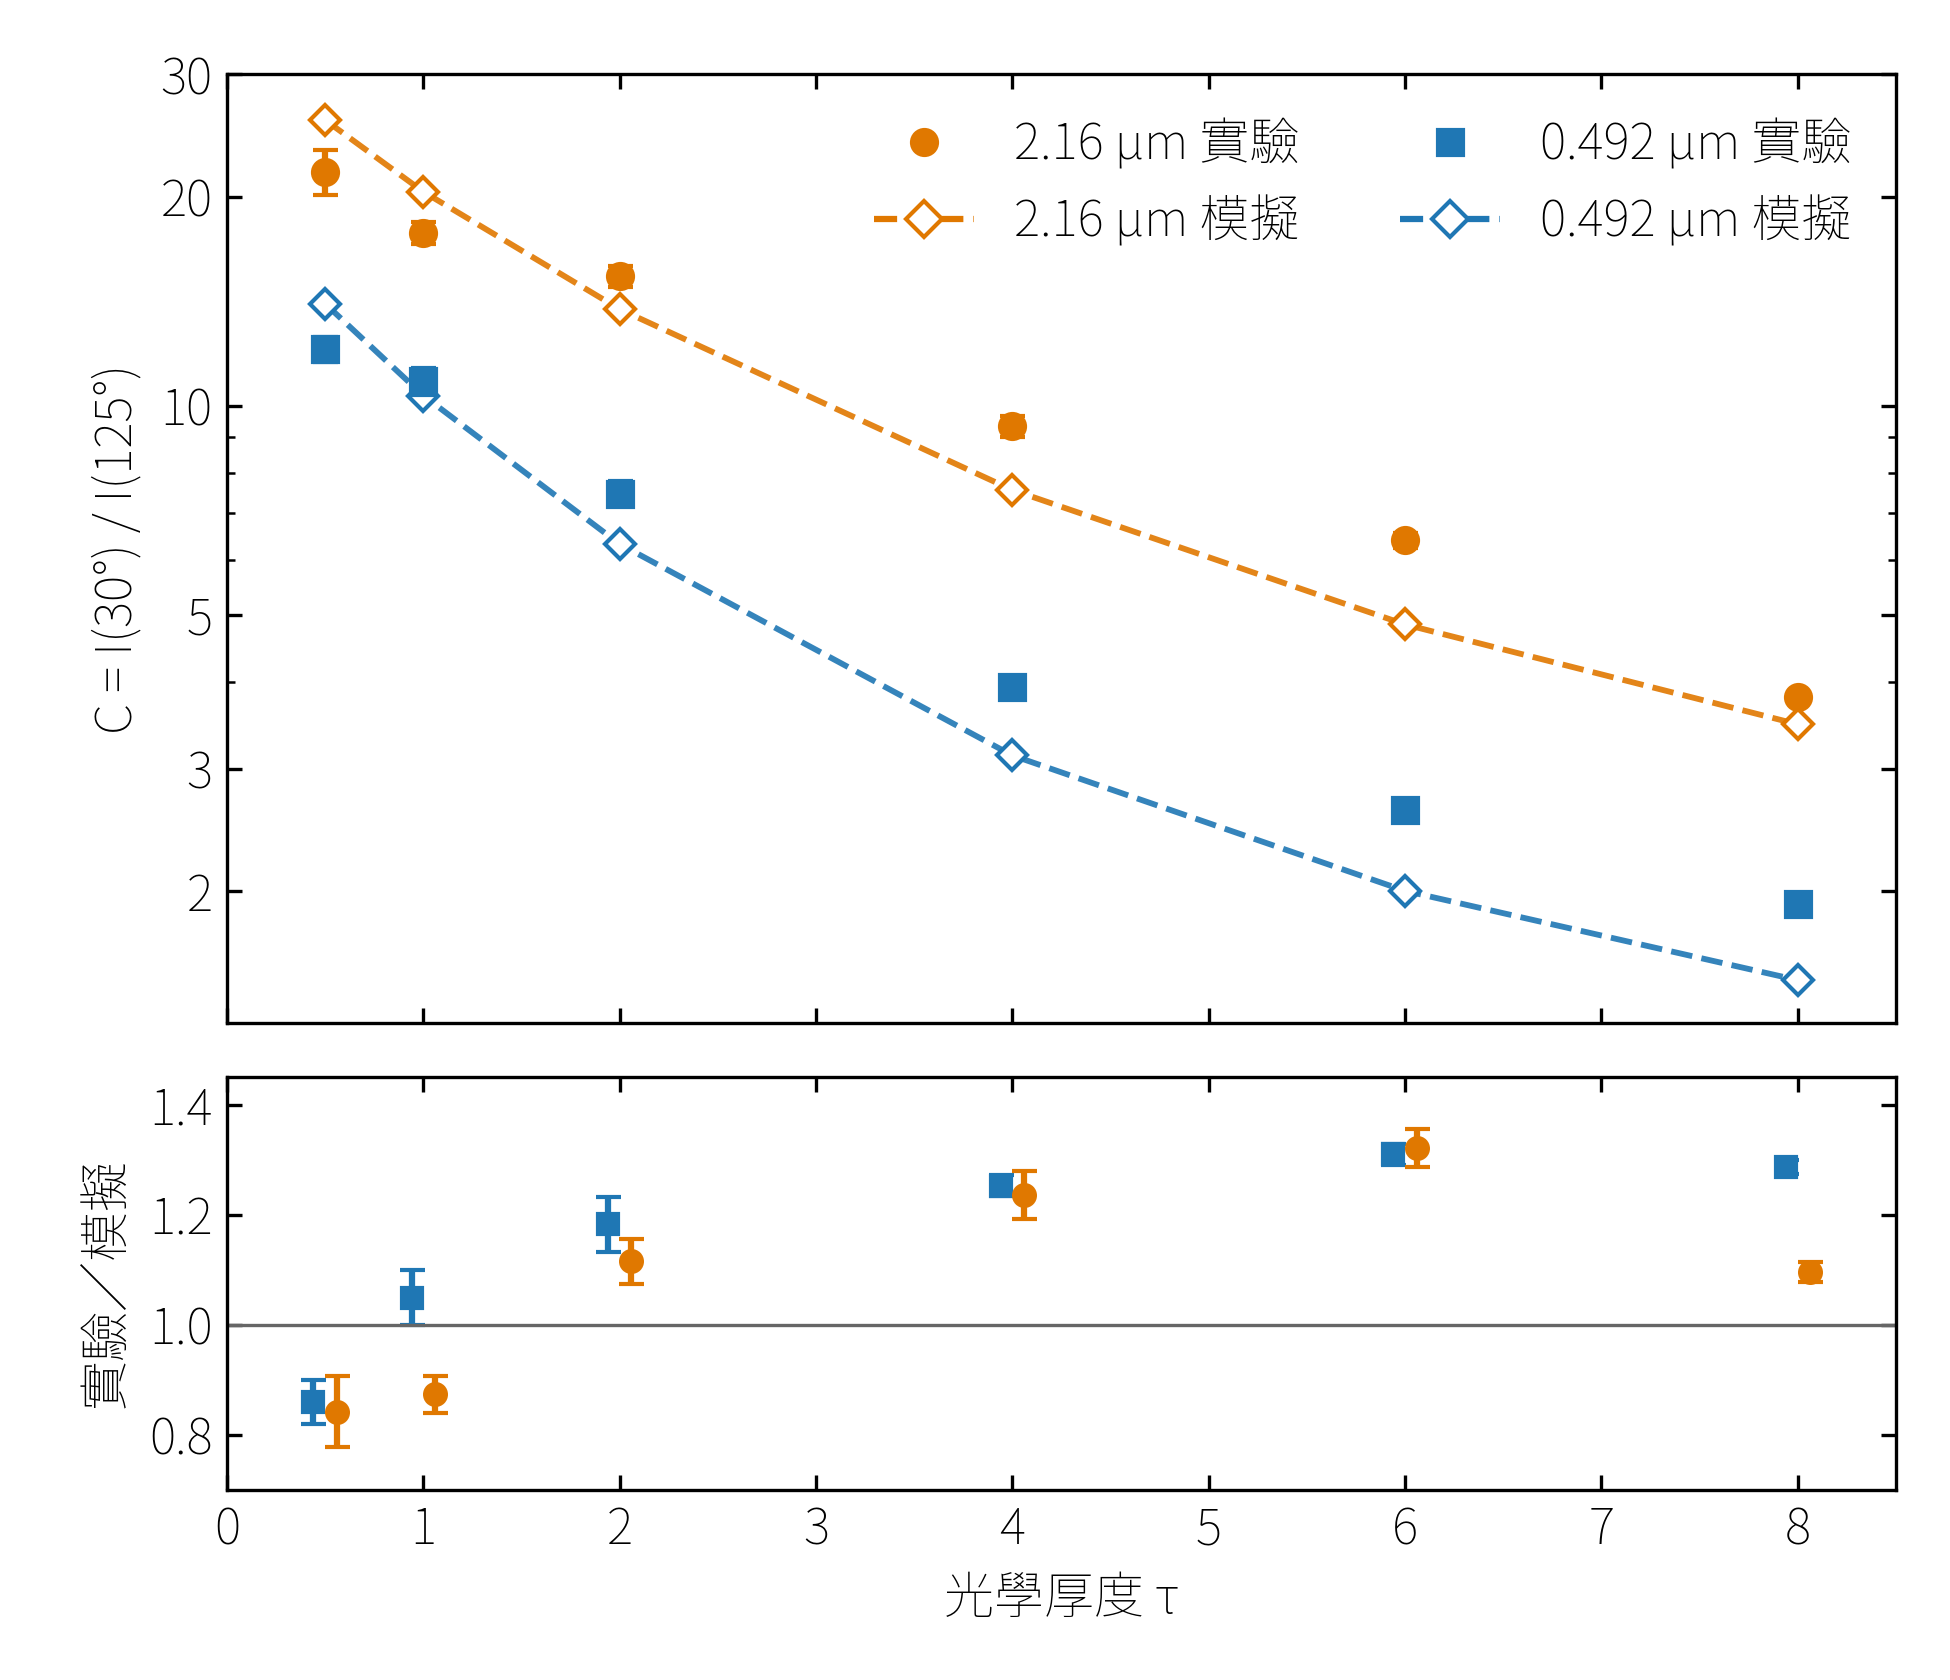
\includegraphics[width=\linewidth]{image/result_C_tau.png}
    \caption{$C$ 隨光學厚度 $\tau$ 的變化。上：實心點為 10 月 24 日實驗值，誤差棒為合成不確定度（$1\sigma$）；空心菱形與虛線為蒙地卡羅模擬（6 組亂數種子平均）；縱軸為對數。下：實驗／模擬比值。}
    \label{fig:C-tau}
\end{figure}

\begin{figure}[H]
    \centering
    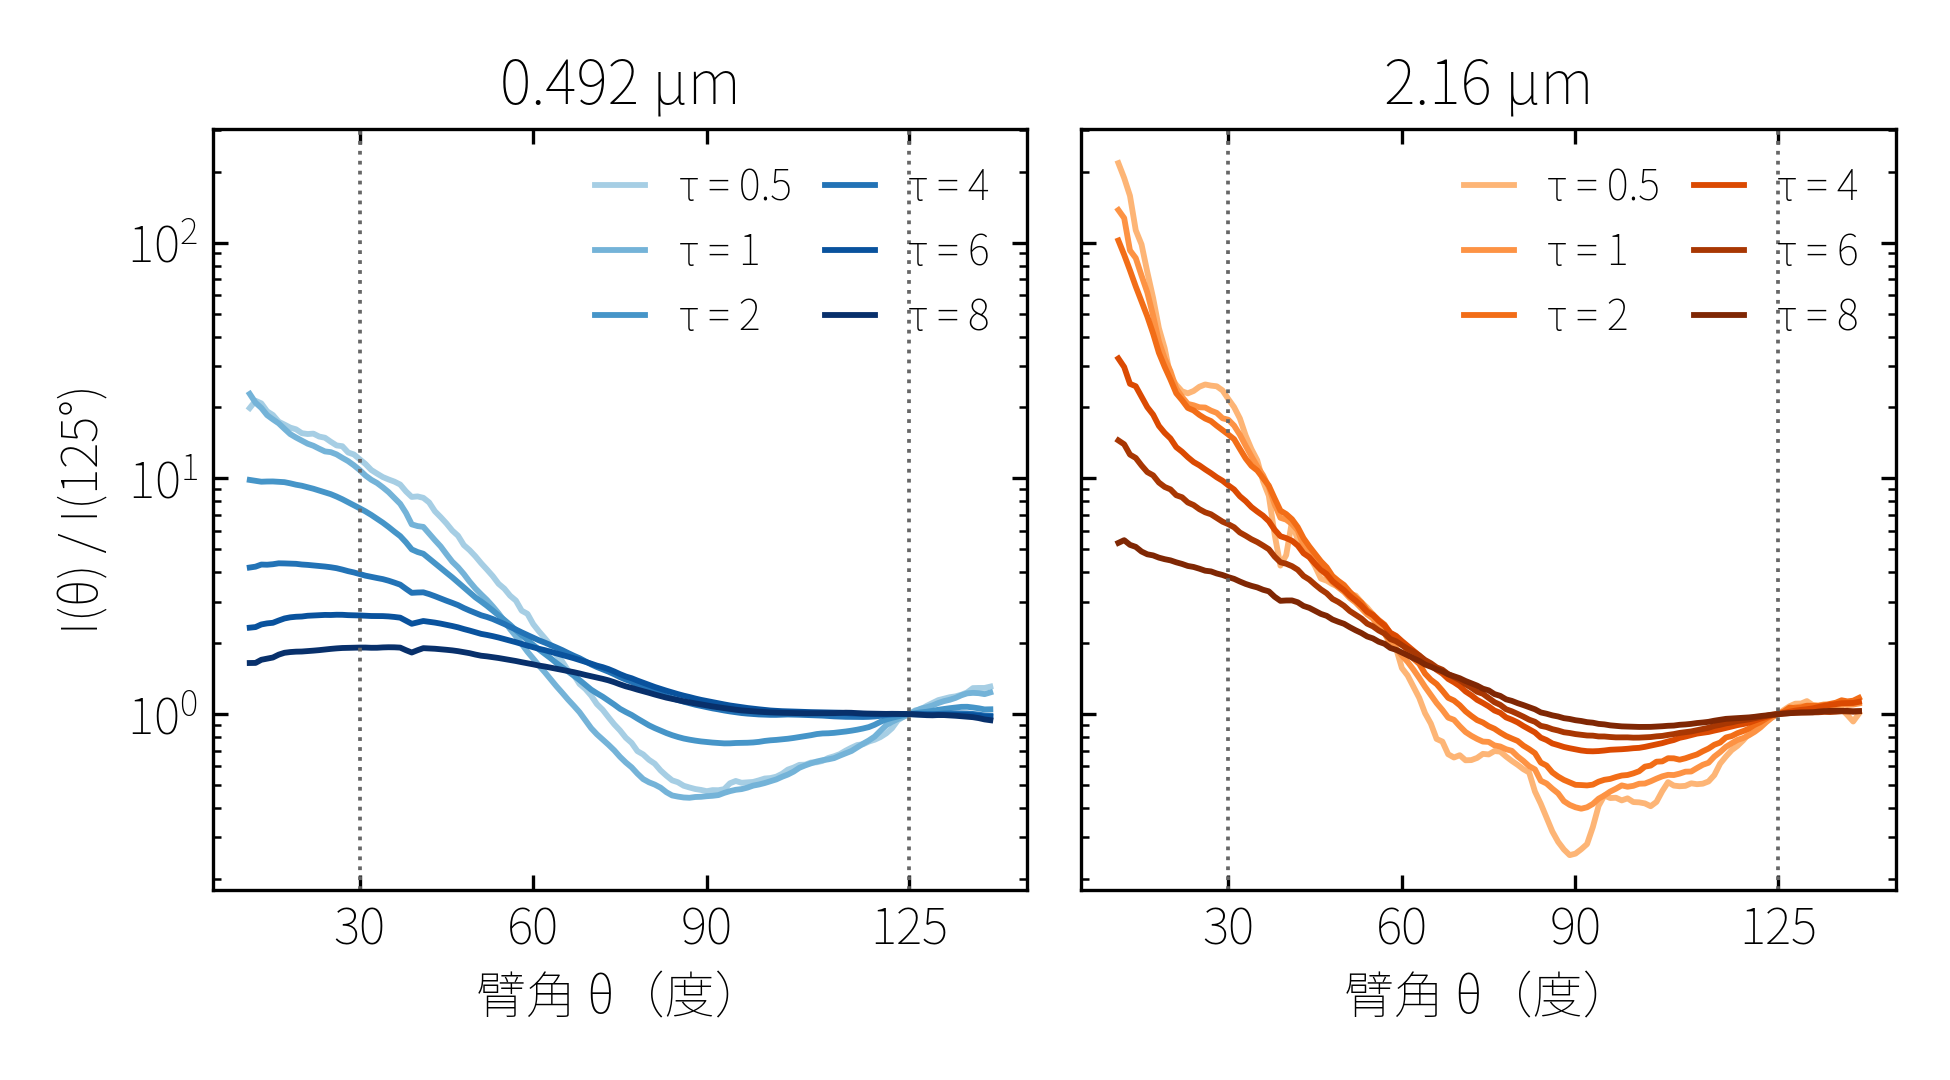
\includegraphics[width=\linewidth]{image/result_Itheta.png}
    \caption{兩種粒徑在不同 $\tau$ 下的實驗角度分布 $I(\theta)/I(125^\circ)$。顏色由淺至深表示 $\tau=0.5$、$1$、$2$、$4$、$6$、$8$；虛線標示 $30^\circ$ 與 $125^\circ$，前者的值即為 $C$。}
    \label{fig:Itheta}
\end{figure}

\begin{figure}[H]
    \centering
    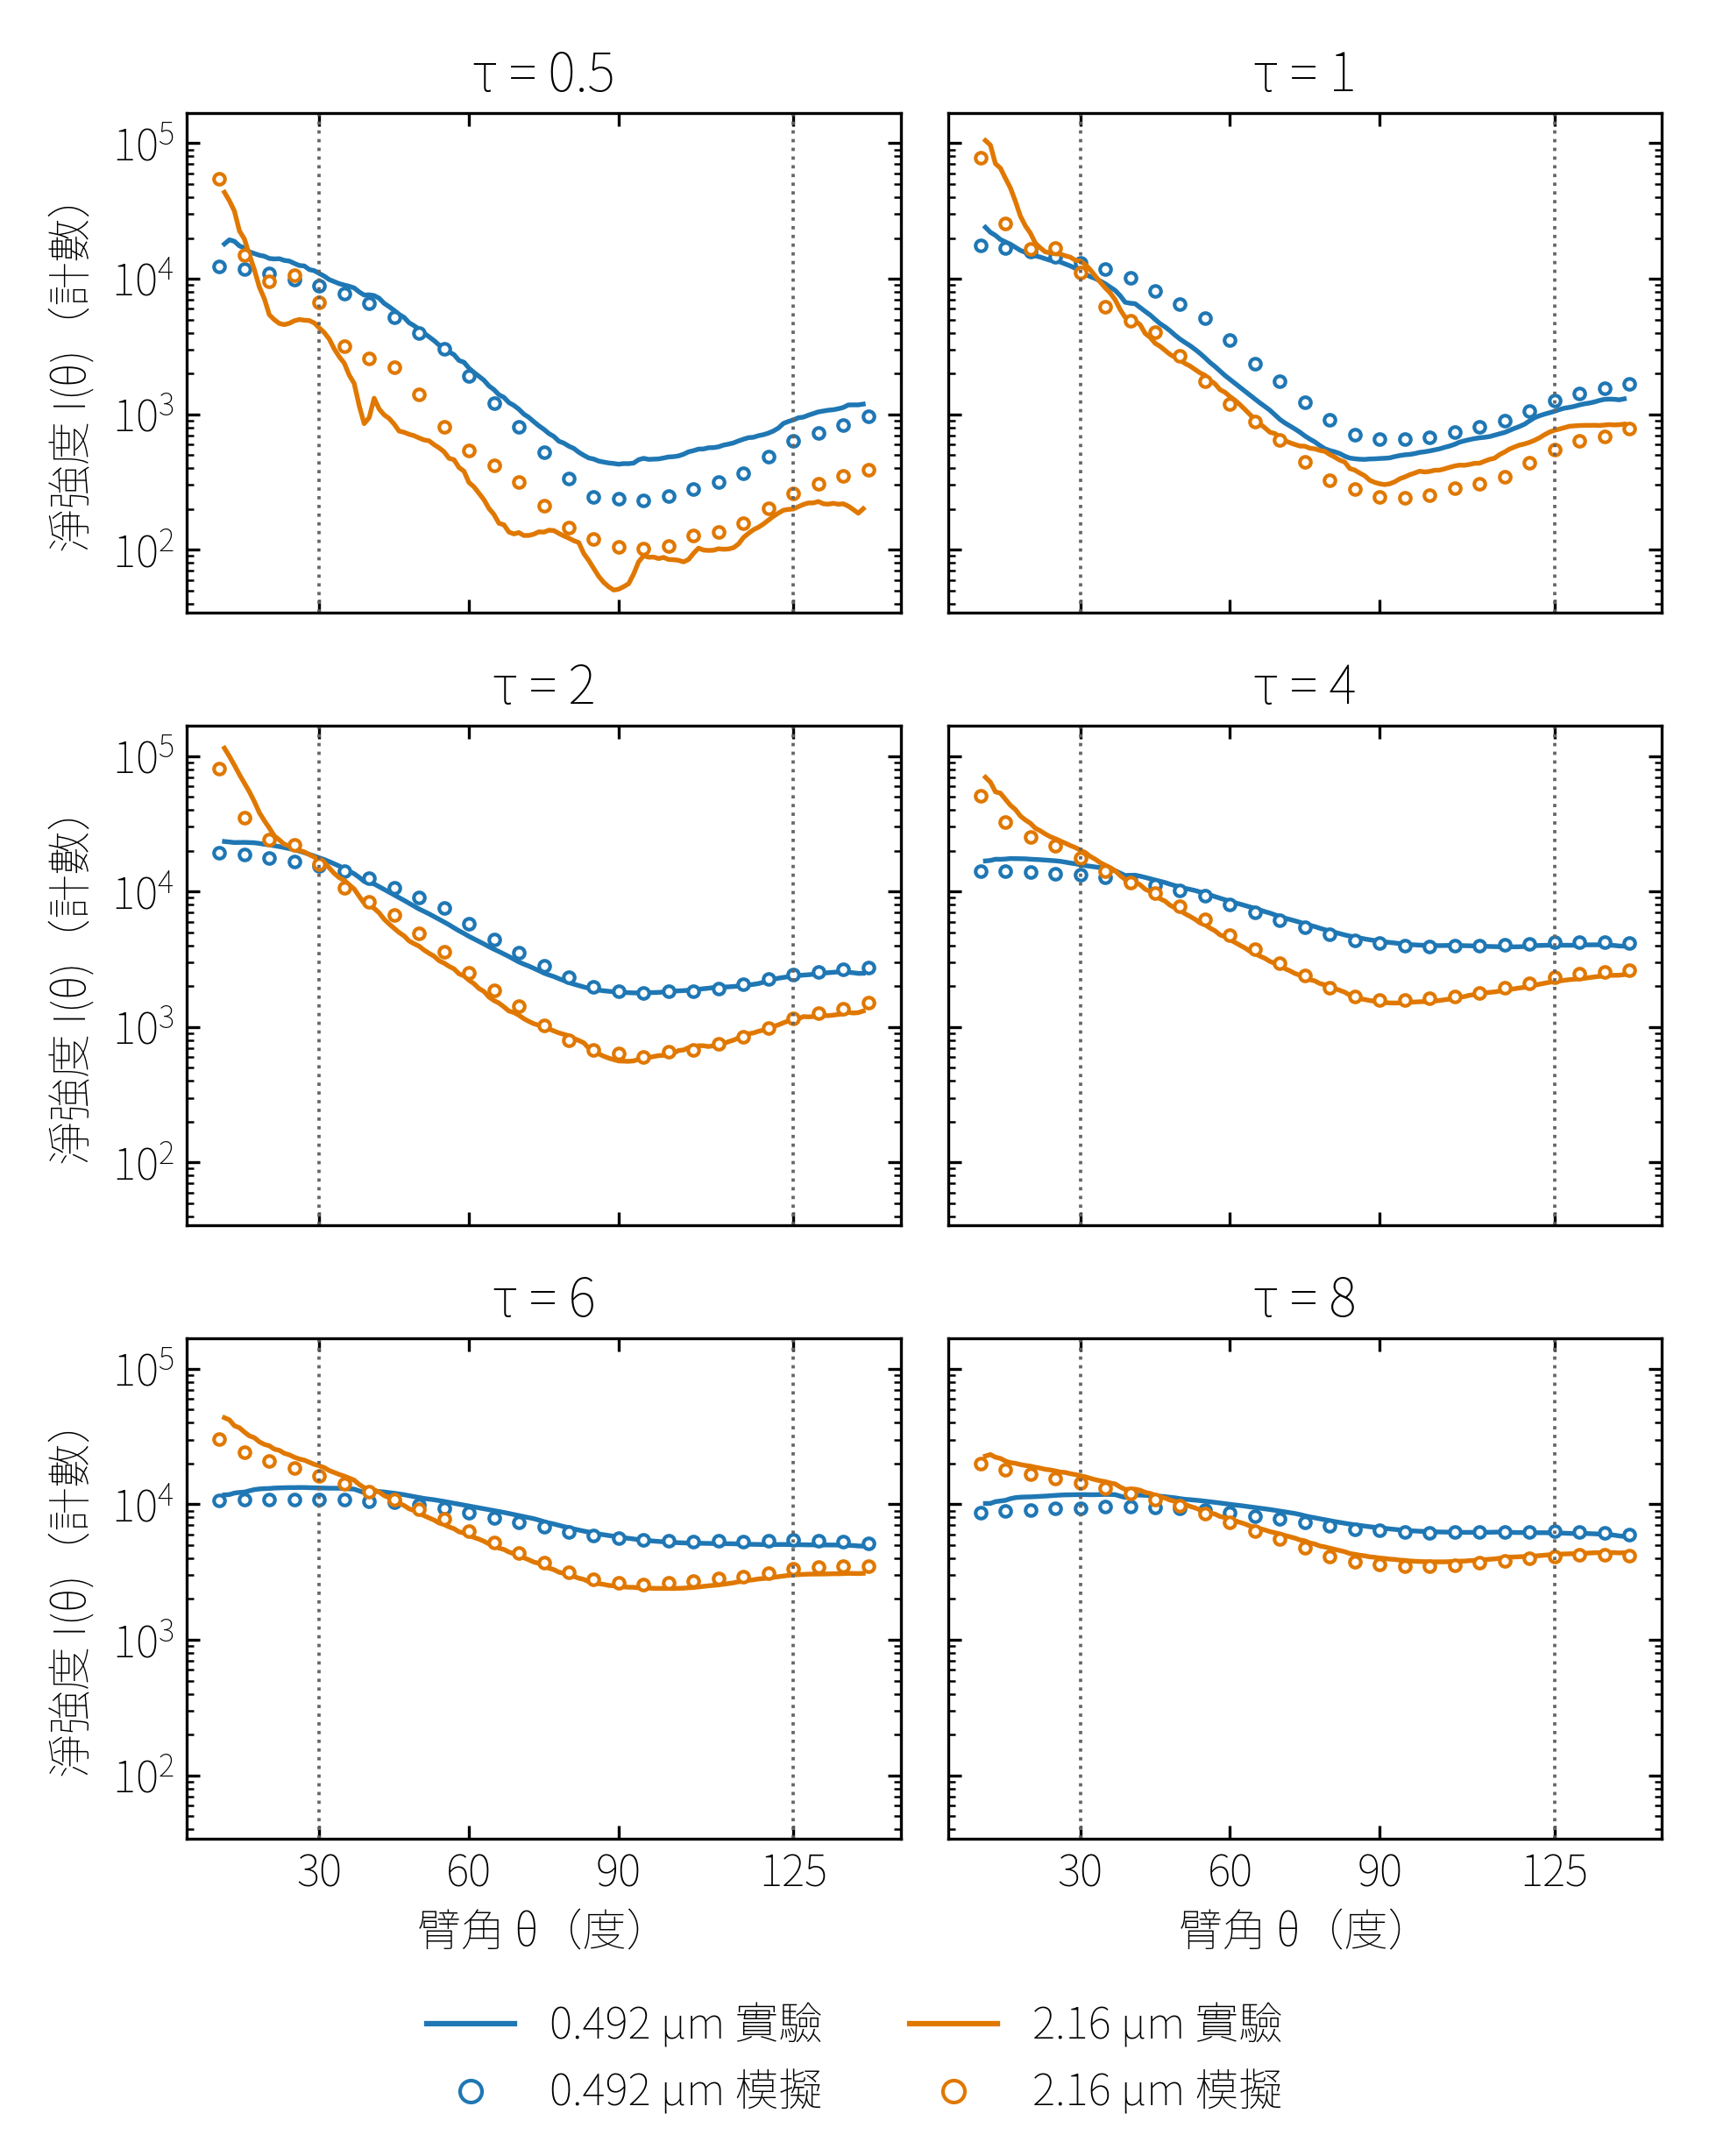
\includegraphics[width=\linewidth]{image/result_abs.png}
    \caption{六個光學厚度下的散射光淨強度 $I(\theta)$。實線為實驗感測器計數，空心圓為蒙地卡羅模擬（$5^\circ$ 一格）乘上共用儀器倍率 $k=2.71\times10^7$；點線標示 $30^\circ$ 與 $125^\circ$。}
    \label{fig:abs}
\end{figure}

\begin{figure}[H]
    \centering
    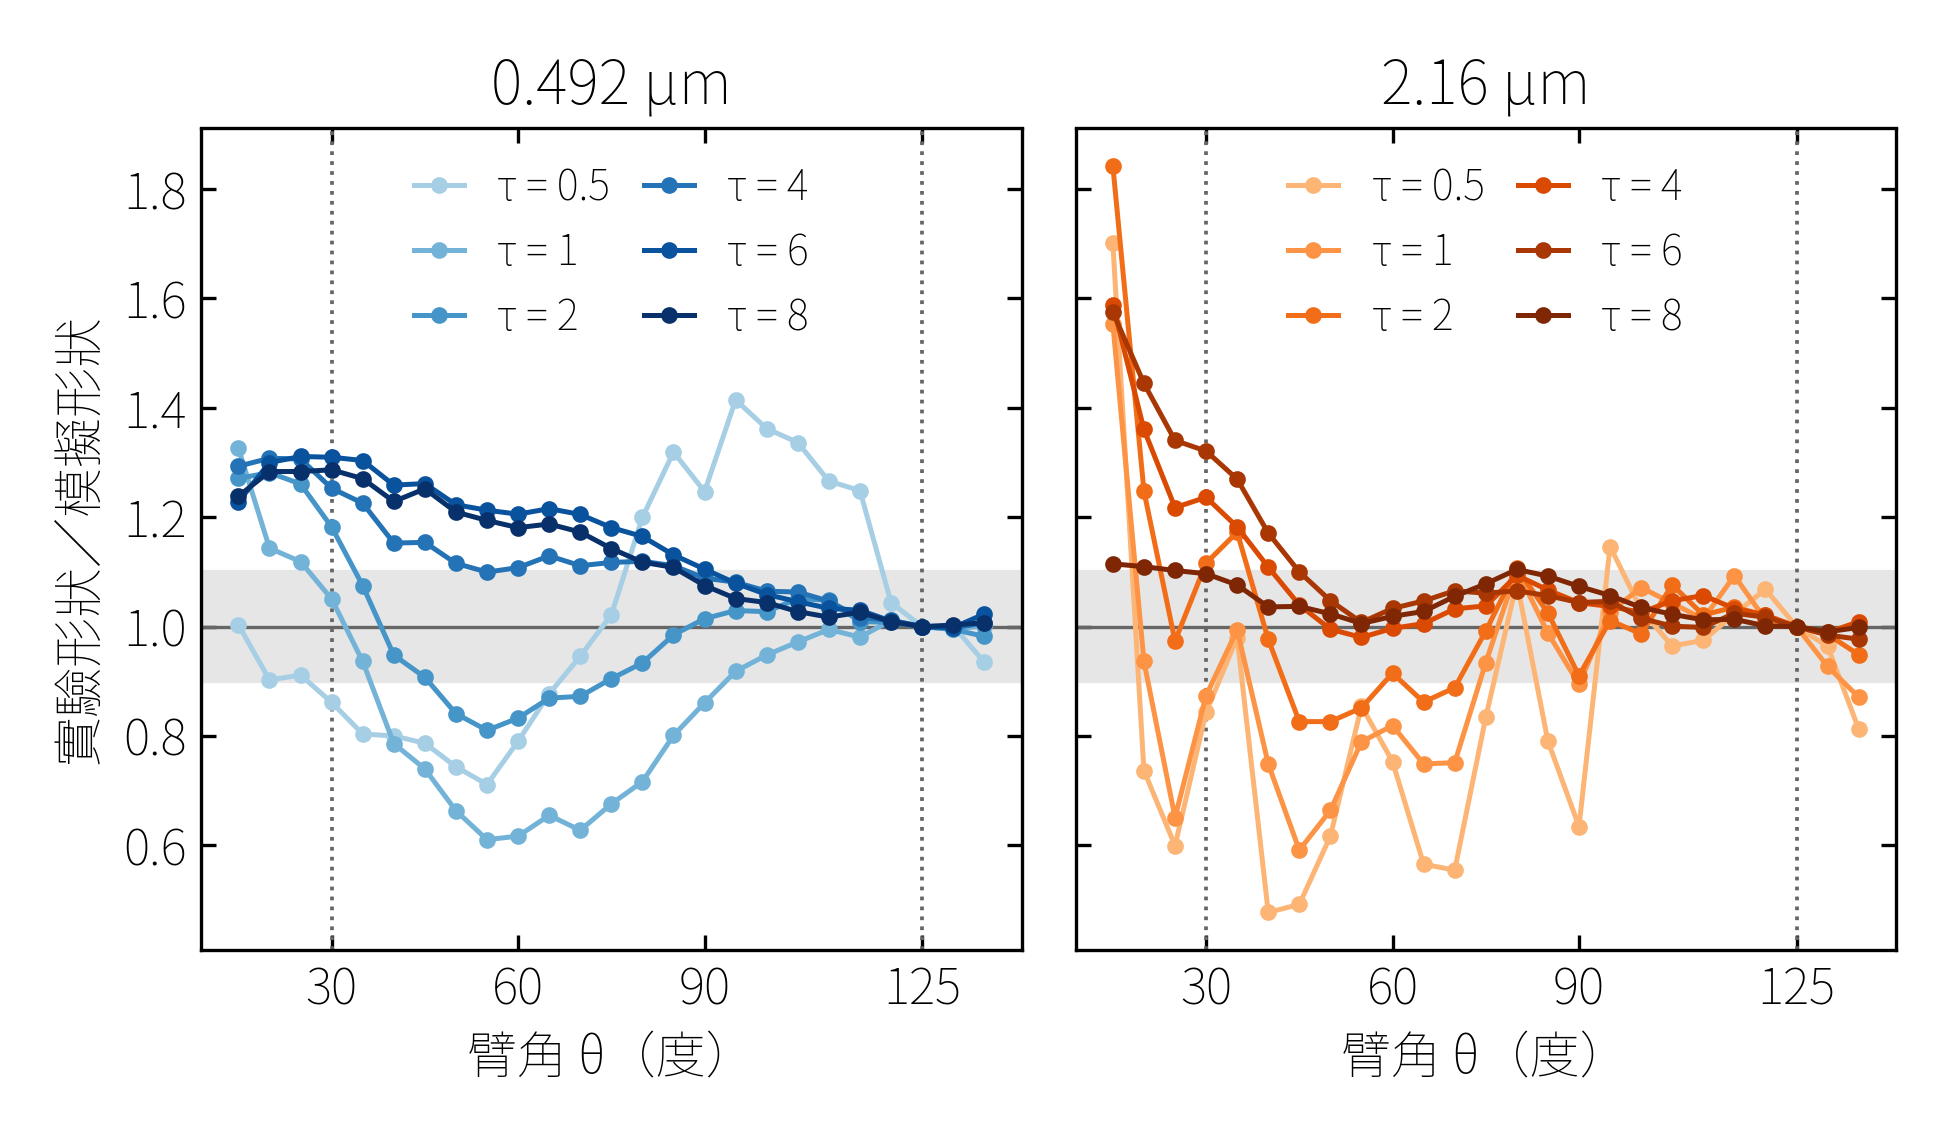
\includegraphics[width=\linewidth]{image/result_shape.png}
    \caption{實驗與模擬角度分布的形狀比 $[I_{\mathrm{exp}}(\theta)/I_{\mathrm{exp}}(125^\circ)]/[I_{\mathrm{MC}}(\theta)/I_{\mathrm{MC}}(125^\circ)]$。$\theta=30^\circ$ 的值即為表~\ref{tab:result-c} 的實驗／模擬比；灰帶為 $1\pm0.1$。}
    \label{fig:shape}
\end{figure}
